\chapter{Modelo de minería de datos}

La necesidad de comprender los procesos biológicos que están implicados en las distintas enfermedades, a partir de la gran cantidad de datos biológicos que hay disponibles como las secuencias genómicas, los microarreglos, las interacciones proteicas, las imágenes biomédicas entre otros. Además la rápida adopción de las historias clínicas electrónicas proporciona una oportunidad de realizar investigaciones a gran escala. Por lo tanto las técnicas de minería de datos para el descubrimiento de conocimiento a partir de la obtención de información proveniente de diferentes fuentes son cada vez mas importantes en la investigación biológica y médica \cite{Wang2017}.\\

El mayor reto de la minería de datos genómicos esta en la extracción de información relevante de grandes volúmenes de datos clínicos y transformarlos en conocimiento, los mayores retos están en: a) La recolección de los datos clínicos y genómicos, b) recuperación de información relevante de datos y c) extracción de nuevos conocimientos de la información \cite{Farid2016}. \\  

Este capitulo esta organizado en análisis exploratorio de los datos que se describe en la sección 5.1, el siguiente, es el analisis textual de información clínica que es discutido en la sección 5.2 en este apartado se describe el analisis de asociación de variantes con la información clínica. Finalmente, el apartado de 5.3 se presentan las conclusiones junto con el resumen del capitulo. 

\section{Análisis exploratorio de los datos.}

Se realizo el análisis exploratorio de la información contenida dentro de la base de datos.Se tomo una muestra de 250 pacientes donados por el laboratorio Genetix S.A.S de los cuales solo 228 contaban con consentimiento informado para utilizar la información con fines de investigación.\\

Los datos fueron consultados desde la base de datos diseña en el cápitulo anterior y fue gestionada con la librería de python pandas \cite{mckinneypandas}. Obteniendose los siguientes resultados:

\begin{figure}[h!]
	\centering
	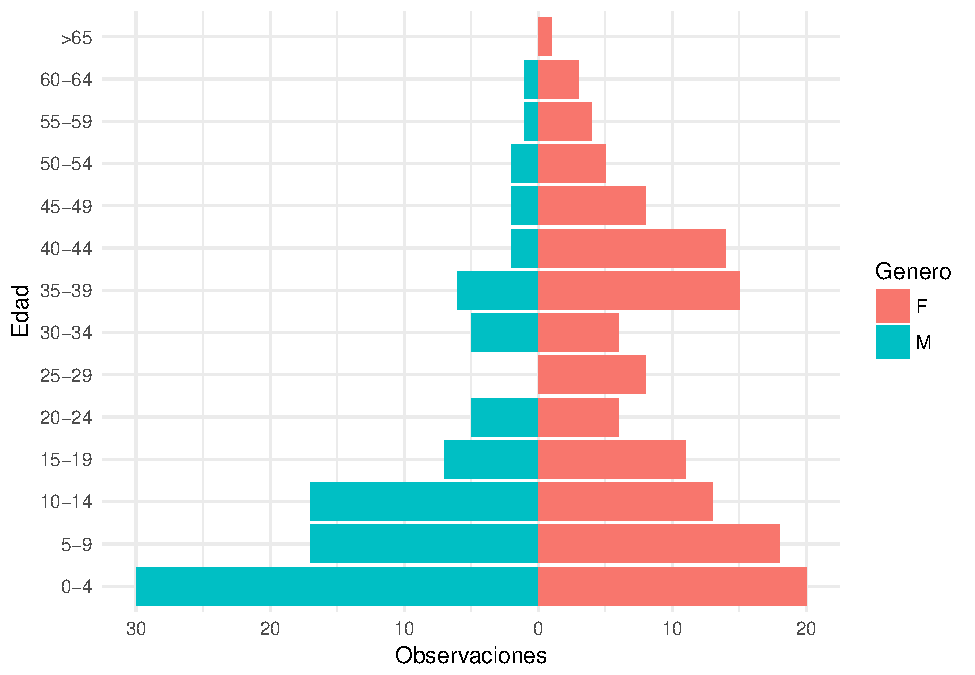
\includegraphics[width=0.5\textwidth]{Kap4/general}
	\caption{Distribución de rango de edades y géneros de los pacientes}
	\label{fig:general}
\end{figure}

\begin{figure}[H]
	\centering
	\subfigure[Distribución de variantes según su tipo.]{
		\label{f:generosgeneral}
		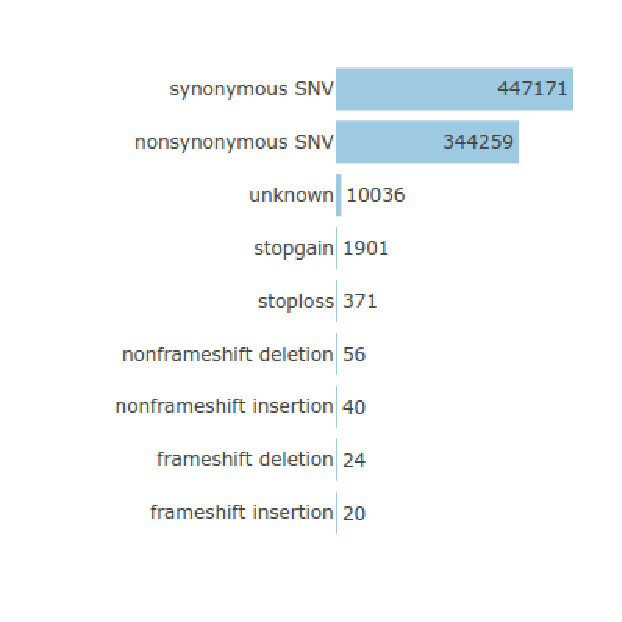
\includegraphics[width=0.35\textwidth]{Kap4/variantes.png}}
	\subfigure[Distribución de variantes por rango de edad]{
		\label{f:variantedad}
		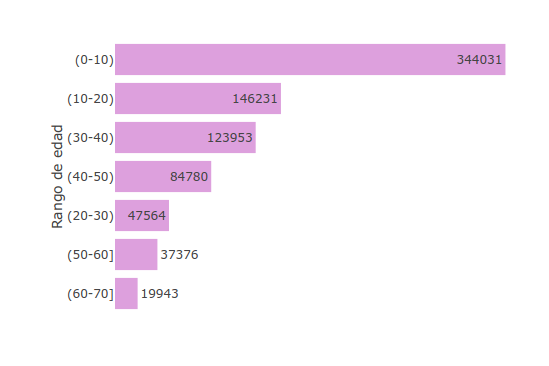
\includegraphics[width=0.55\textwidth]{Kap4/edad.png}}
	\caption{Distribución del tipo de variantes}
	\label{f:variantesgeneral}
\end{figure}

La base de datos contiene 228 pacientes de los cuales 133 son de género femenino y tienen un total de 468.485 variantes y 95 de género masculino con 345.239 de variantes obteniendo  un total de 803.878 variantes. La  figura \ref{fig:general} representa la distribución de pacientes por rango de edades y la figura \ref{f:variantesgeneral} representa la distribución de variantes según su tipo. En la figura \ref{f:generosgeneral} muestra el número de variantes que son sinónimas y no sinónimas siendo las más frecuentes en la población, a  nivel mundial se conoce que estos son lo tipos de variantes más frecuentes\cite{Fu2013}.\\

Las variantes desconocidas son el tercer tipo de variante más frecuente dado que aún existe el problema de selección del transcripto para realizar la nomenclatura adecuada de las variantes, por lo que el anotador informa que son desconocidas \cite{McCarthy2014}. La figura\ref{f:variantedad} muestra la distribución de las variantes identificadas según el rango de edad, siendo el rango con mayor número de variantes los pacientes que se encuentran entre las edades de 0 a 10 años, dado a que es la población más representada dentro de la base de datos. \\

El estado alélico de las variantes (cigocidad) que se encuentran dentro de la base de datos se dividen en heterocigotas 458639 que corresponden al 57,05\% del total de las variantes  y homocigotas 345239 que corresponden al 42,95\%. La distribución de la cigocidad de las variantes se puede explicar desde el error que se puede generar en la identificación de las variantes dado que durante el llamado  de variantes es posible que una variante homocigota se catalogue como heterocigota o si durante el proceso de secuenciación se identifican erróneamente los nucleótidos \cite{Babraham2016}\cite{Pirooznia2014}. 


\section{Análisis textual de información clínica.}

 
\subsection{Preprocesamiento.}

El proceso de limpieza y nacionalización de texto se realizo de la siguiente manera:

 \begin{enumerate}
 	\item Remoción de stop words en español, tildes y caracteres especiales como  la letra ñ y todos los documentos se unificaron en letras minúsculas.
 	\item Teniendo en cuenta la información clínica se creo un diccionario de sinónimos, donde se reemplazaron palabras que hacen referencia a una misma característica.
 	\item Calculo de la frecuencias de palabras dentro de los documentos. 
 	\item Se removieron las palabras pam,pacientes, secuenciación y gen dado que no son un factor diferenciador de los documentos.  	  
 \end{enumerate}

\subsection*{Resultados}

Los resultados que se obtuvieron para la frecuencia de palabras fueron seno, cáncer, síndrome, sospecha y años. La figura \ref{fig:sin} muestra las primeras 30 palabras más frecuentes y la nube de palabras de todos los documentos.\\

\begin{figure}[]
	\centering
	\subfigure[Nube de palabras]{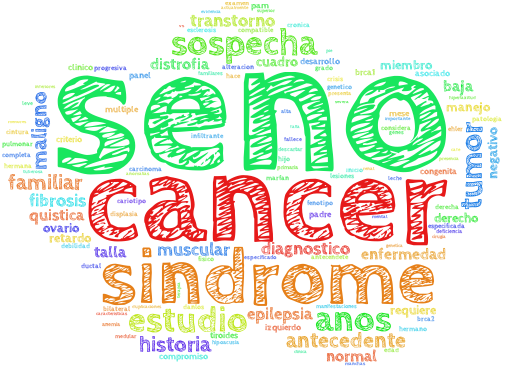
\includegraphics[width=60mm]{Kap4/sin_stop}}
	\subfigure[Frecuencia de términos]{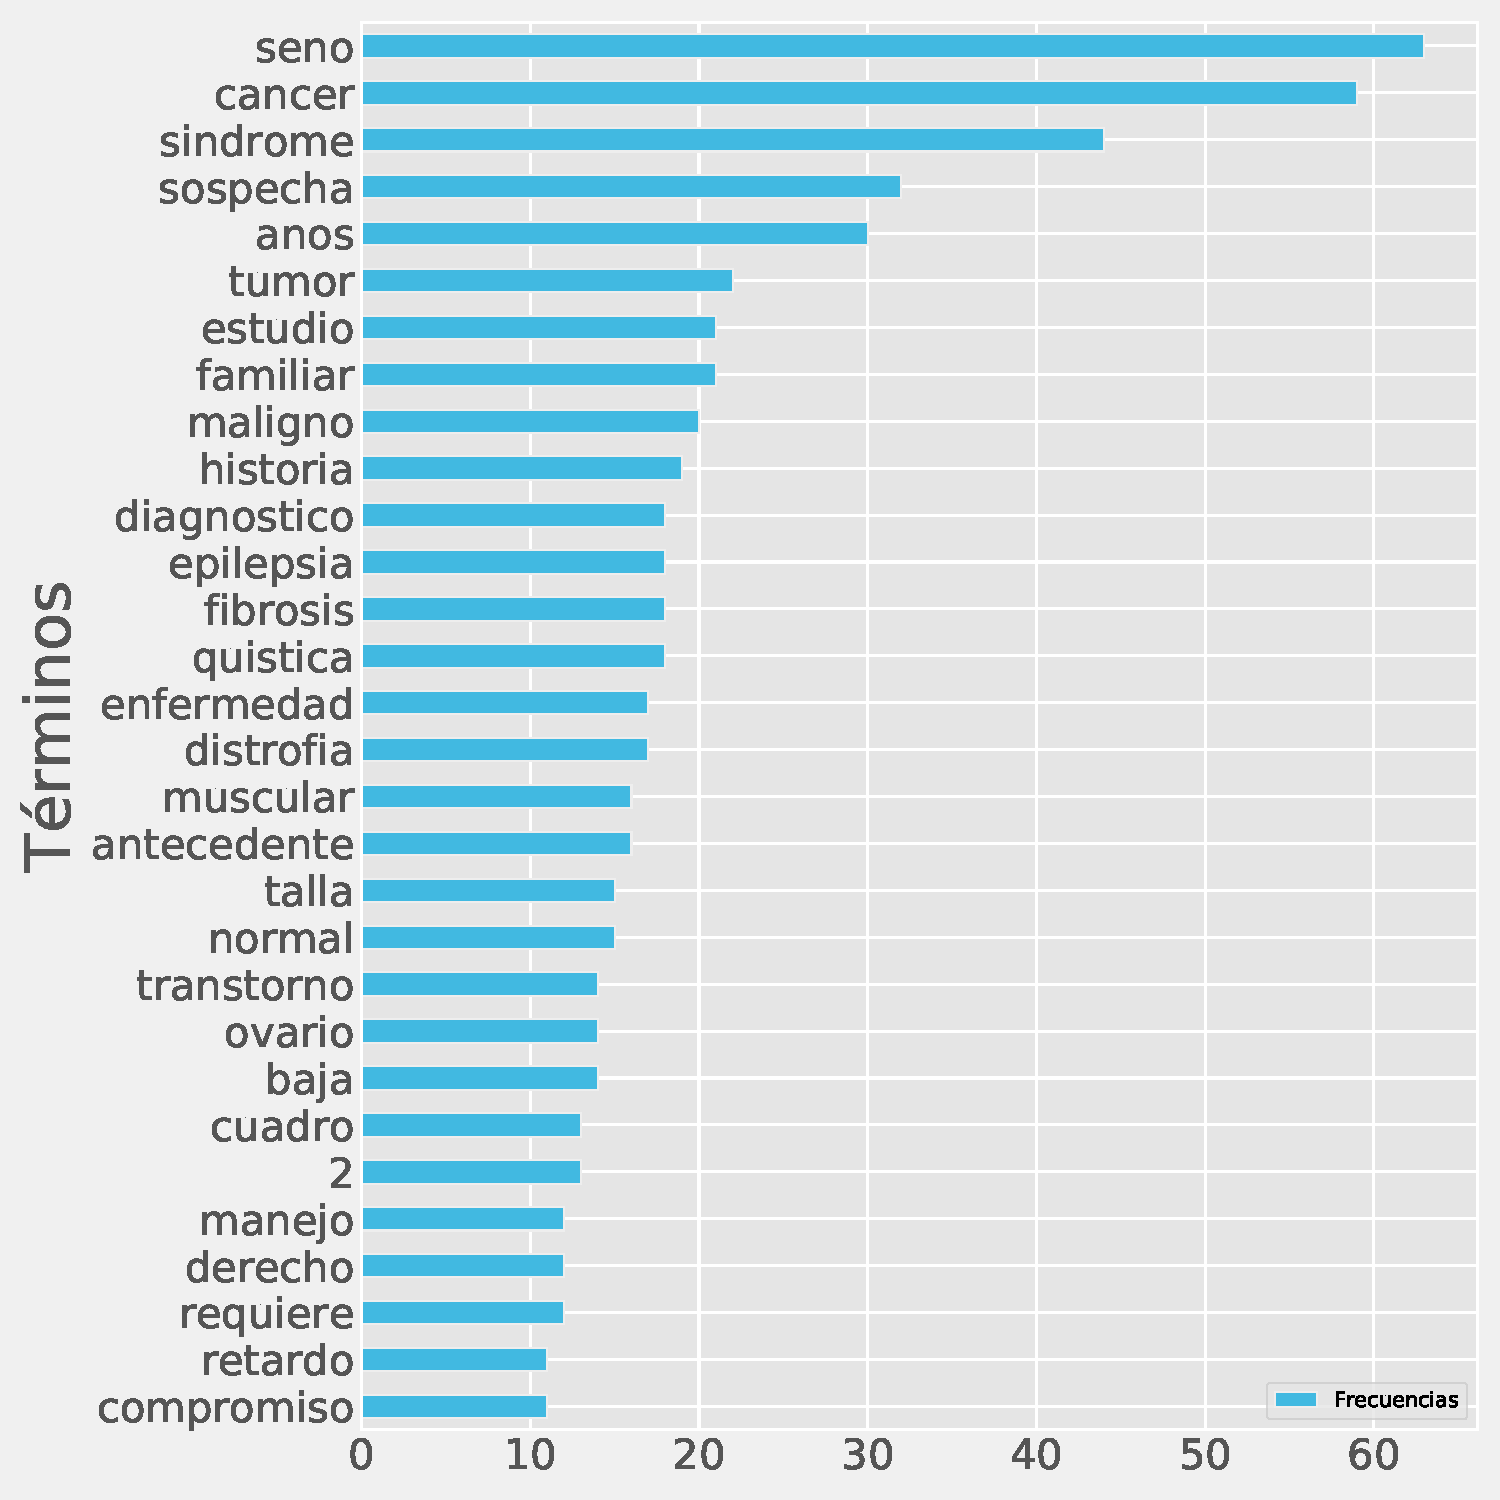
\includegraphics[width=60mm]{Kap4/frecuecias.pdf}}
	\caption{Frecuencias sin stop words y palabras sinónimas} \label{fig:sin}
\end{figure} 

Las frecuencia de palabras nos muestra las principales características de la información clínica siendo las palabras cáncer y seno los principales fenotipos, también se encuentra la palabra síndrome que puede asociarse a diferentes  enfermedades y la palabra sospecha hace referencia a diagnósticos ambiguos que pueden tener los pacientes, una de las contribuciones de la secuenciación es que basado en el fenotipo puede ayudar a un diagnóstico,entre diferentes síntomas y síndromes que pueden ser aplicados a enfermedades raras y complejas\cite{Tetreault2015a}.

\subsection{Grupos de características clínicas.}

En los procesos médicos, la relación entre los factores que pueden afectar la salud juega un papel importante. Una de las relaciones más comunes es la relación entre los genes y las enfermedades donde la secuenciación de exones tiene una alta aplicabilidad. Pero la identificación manual de este tipo de relaciones es compleja dada la cantidad de características que se pueden presentar como el diagnóstico propio de la enfermedad y/o la respuesta a los tratamientos \cite{Kawashima2017}.\\

La minería texto y puede ser aplicado al análisis en la medicina, donde el clustering (agrupamiento) puede ser considerado el método más importante que se utiliza en aprendizaje de maquina no supervisado que ha sido aplicado a diferentes problemas\cite{Kawashima2017}, teniendo en cuenta que no de los objetivos del agrupamiento de datos, es la  identificación de grupos naturales en datos sin etiquetas\cite{Jain2010}.\\

Partiendo de lo anterior el presente trabajo se implemento un modelo de agrupamiento utilizando el kmeans  para identificar grupos de características clínicas con la siguiente metodología:

\begin{enumerate}
	\item Cálculo de la matriz tf-idf y se normalizo. 
	\item Estimación de el número de k optimo.
	\item Implementación del algoritmo k-means.
	\item Validación de los clusters.
	\item Análisis de resultados. 	  
\end{enumerate}

\subsubsection{Transformación de los datos.}

El cálculo de la matriz tf-idf, se realiza a partir de frecuencia invertida con la ecuación 
$${idf}_i = \log_2 \frac{|D|}{|\{d \mid t_i \in d\}|}$$
siendo $|D|$ lo que denota el número total de documentos y donde $|\{d\mid t_i \in d\}|$ en  que $t_1$ aparece, la matriz de tf-idf es calculada a partir de la multiplicación de la frecuencia de términos y la frecuencia invertida $\mathit{tf}_{i,j} \cdot \mathit{idf}_i$ \cite{Buckley1988}. 
La figura \ref{fig:IDFTF} representa la matriz IDF-TF de las palabras que se encuentran dentro de la base de datos.  

\begin{figure}[H] 
	\centering
	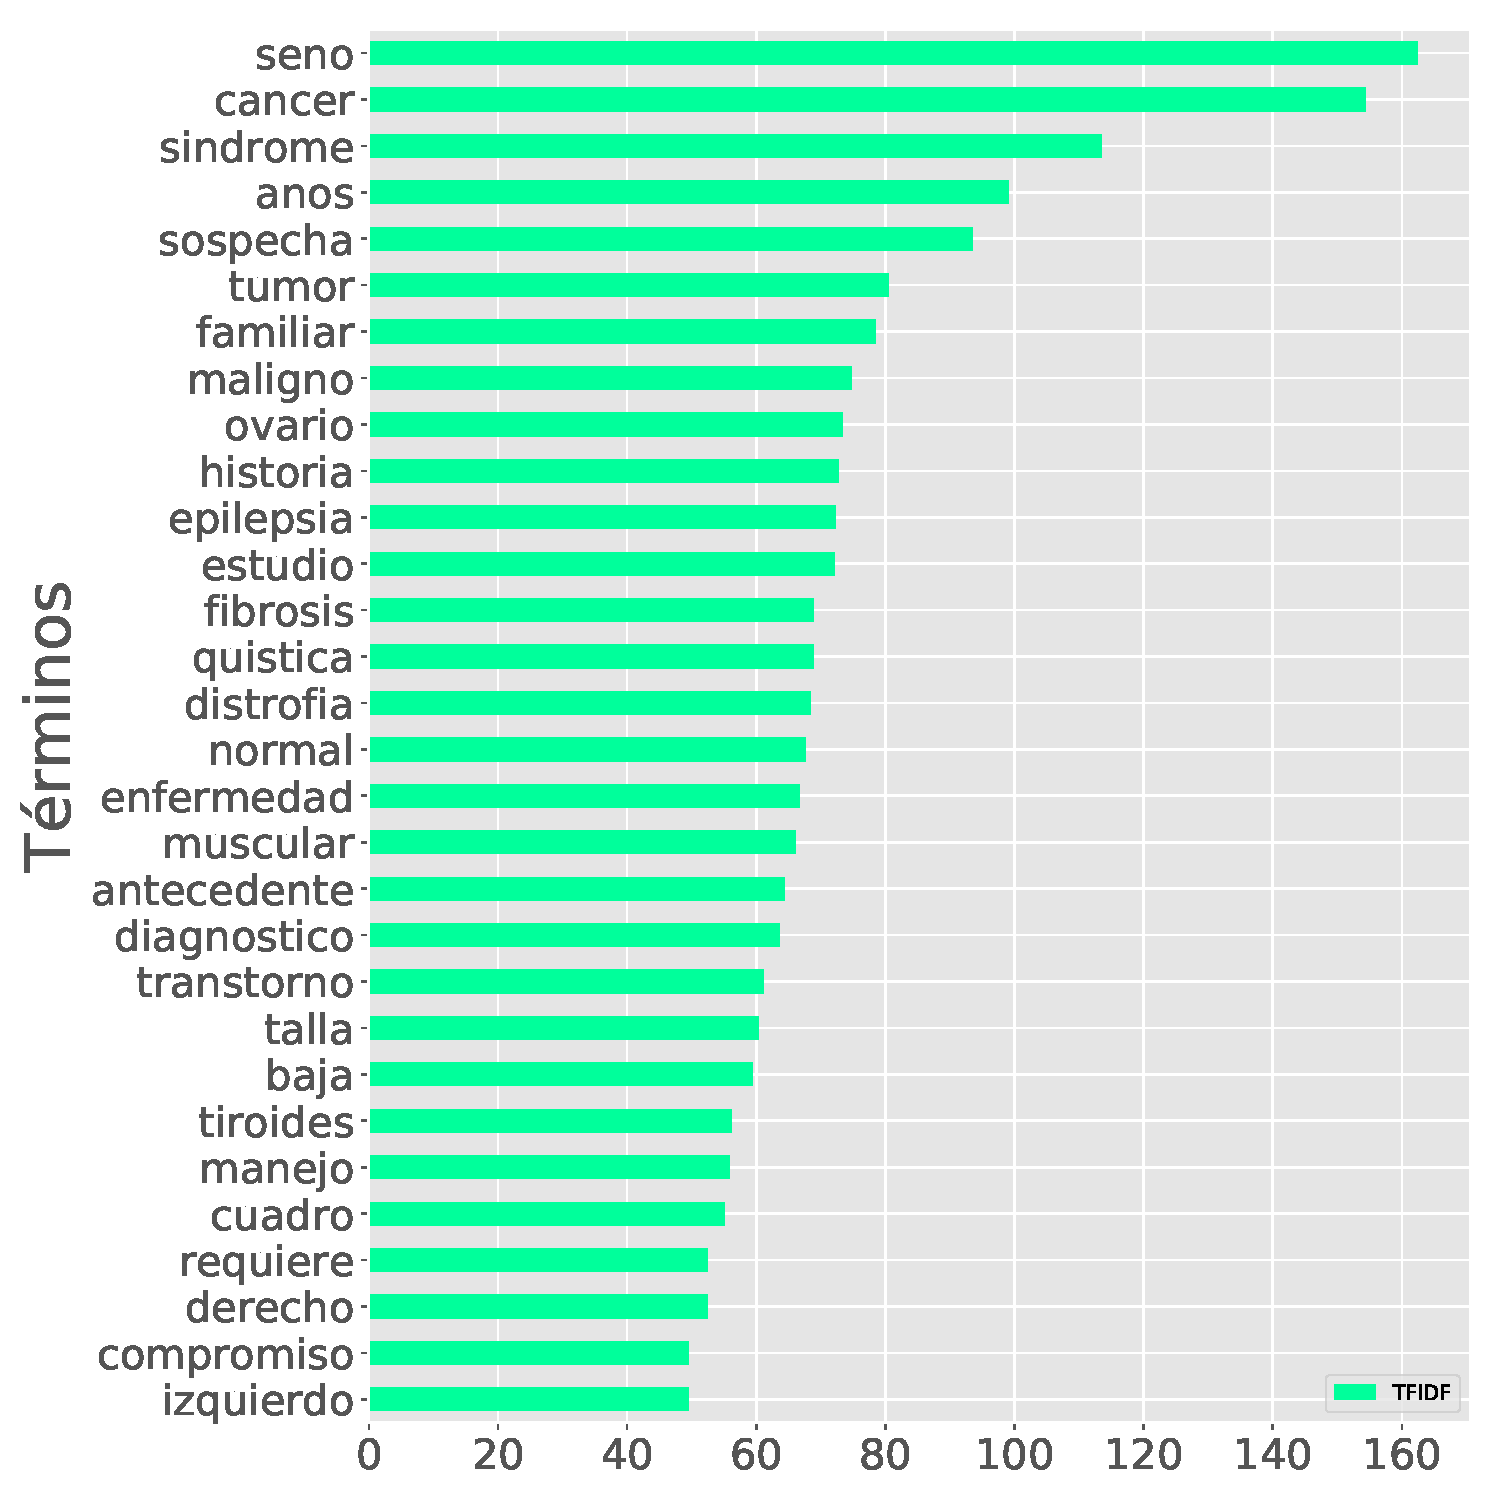
\includegraphics[width=0.5\textwidth]{Kap4/tfidf.pdf}
	\caption{TF-IDF} 
	\label{fig:IDFTF}
\end{figure}

Una vez obtenida la matriz tf-idf se normalizo y se le aplico la similaridad de coseno que es una de las medidas más populares para aplicar en documentos de texto. Esta medida tiene como ventaja que es independiente del largo del documento \cite{Huang2008}.Esta similitud fue computada de acuerdo a la siguiente formula donde la similitud ente $u$  y $v$ es definida como  según la librería scipy de python \cite{scipy}, Donde posteriormente los datos fueron utilizados para el clustering:
$$   1 - \frac{u \cdot v}
{||u||_2 ||v||_2}. $$

donde $u.v$ donde el punto es el producto de $u$ y $v$.

\subsubsection{Validación del modelo de clustering.}

La selección del número óptimo de $K$ se realizo utilizando el método del codo, este es uno de los métodos más antiguos para determinar el número de de cluster, se realizan varios experimentos iniciando por un $K$ = 2 y realizando un incremento de 1, para los cuáles se calcula el costo que conlleva cada una de las ejecuciones; entre más se aumente el número de $K7$ el costo disminuye y el número de $K$ alcanza una meseta, este valor es el que se desea obtener, visualmente se realiza la identificación mediente un gráfico de error cuadrático y número de clusters , la razón es que al continuar el aumento del número de K los nuevos clusters son muy cercanos a otros ya generados \cite{Kodinariya2013}.\\   

El cálculo del error cuadrático vs el número de clusters se realizo utilizando la libreria de python scikit learn, donde se computa el valor de la inercia que es calculada como la suma de cuadrados por cada punto cercano al centroide y es asignado al cluster. Así que  $I = \sum_{i}(d(i,cr))$ donde $cr$ es el centroide que fue asignado al cluster y $d$ es la distancia cuadrada \cite{scikit-learn}. 

\begin{figure}[H] 
	\centering
	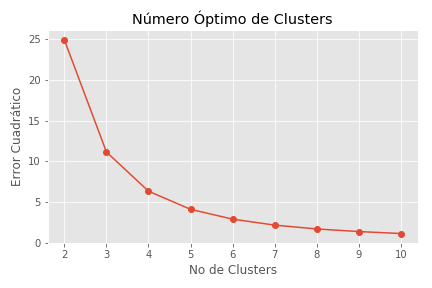
\includegraphics[width=0.5\textwidth]{Kap4/Clusters}
	\caption{Número optimo de clusters} 
	\label{fig:Clusters}
\end{figure}

Una vez se computo la inercia se realizo genero el gráfico del error cuadrático vs el número de clusters  la figura \ref{fig:Clusters} muestra el gráfico de codo obtenido, donde se puede seleccionar el cluster 5 y 6 como óptimo de $K$.\\

Para definir el número de optimo de $K$ también se computo el coeficiente de Silhouette que es una evaluación de los clusters, donde los valores altos son relacionados a modelos que tienen clusteres bien definidos .El coefiente está definido por cada muestra y está compuesta por dos valores que son \cite{scikit-learn,Rousseeuw1987}:

\begin{itemize}
	\item \textbf{a:} La distancia media entre una muestra y todos los puntos de la misma clase.
	\item \textbf{b:} La distancia media entre una muestra y todos los otros puntos en el próximo cluster más cercano.
\end{itemize}

El coeficiente Silhouette $s$ para una sola muestra se da como:

$$s = \frac{b-a}{max(a,b)}$$

Para un set de datos el coeficiente Silhouette es el promedio del coeficiente por cada muestra \cite{scikit-learn,Rousseeuw1987}. En el presente trabajo los resultados del coeficiente de Silhouette fue de  \textit{0.534}, adicionalmente se gráfico los valores de del coeficiente Silhouette para un $K$ = 5 y se presenta en la figura \ref{fig:S}:

\begin{figure}[H] 
	\centering
	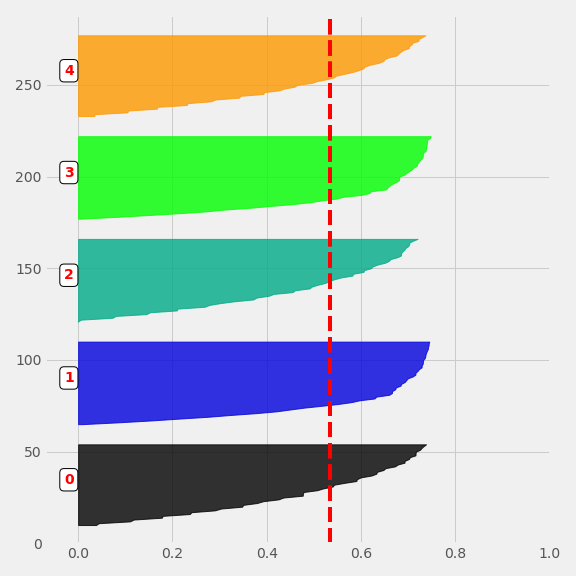
\includegraphics[width=0.3\textwidth]{Kap4/S}
	\caption{Valor Silhouette por cada cluster} 
	\label{fig:S}
\end{figure}

Para los clusters obtenidos se calcularon las medidas de validación que están dentro de la librería scikit-learn \cite{scikit-learn} son:

\begin{itemize}
	\item  \textbf{Homogeneidad:} Definida como donde cada cluster contiene solo datos de una misma clase.
	\item \textbf{Integridad:} Donde todos los miembros de una misma clase son asignados al mismo clúster.	
	\item \textbf{V-measure:} Es la medida armónica ente la homogeneidad y la integridad \cite{Rosenberg2007}. 		
\end{itemize}

El cálculo de la homogeneidad y la integridad del cluster es realizada por:
$$h=1- \frac{H(C|K)}{H(C)} $$

$$c=1- \frac{H(K|C)}{H(K)}$$

donde $H(C|K)$ es la entropía condicional de las clases en cada asignación de cluster y que son calculadas por:

$$H(C|K)= - \sum_{c=1}^{|C|} \sum_{k=1}^{|K|} \frac{n_c,_k}{n} . \log \frac{n_c,_k}{n_k}$$ 

y $H(C)$ es la entropia de clases y es calculada:
$$H(C)=  - \sum_{c=1}^{|C|} \frac{n_c}{n} . \log \frac{n_c}{n}$$ 
con $n$ que es el número total de muestras $n_c$ y $n_k$ son el número de muestras asignadas respectivamente a la clase $c$ y al cluster $k$, y finalmente $n_c,_k$ son el número de muestras de las clases$c$ asignadas al cluster $k$.

Finalmente el V-measure está definido de la siguiente manera \cite{Rosenberg2007}:

$$v= 2.\frac{h.c}{h+c}$$

También se calculo Rand-Index que calcula una medida de similitud entre dos grupos al cosiderar todos los pares de las muestras y los pares de conteo que se asignan al mismo cluster o en diferentes grupos. Calculado de la siguente manera \cite{scikit-learn}:
$$ARI = (RI - Expected_RI) / (max(RI) - Expected_RI)$$

Los resultados de validación obtenidos fueron:

Para homogeneidad 0.296, para integridad 1.0, para el V-measure 0.457 y el Rand-Index fue 0. La homogeneidad perfecta sería con un valor de 1.0, en los presentes clusters presentan una baja homogeneidad, pero una una integridad de 1.0 que significa que las etiquetas son perfectamente completas, esto se ve reflejado en el V-measure que es de 0.457 donde tenemos clusters con baja homogeneidad pero una alta integridad.  Rand-Index se obtuvo un valor de 0.0 que muestra que las clases están separadas en diferentes clusters \cite{scikit-learn}. 

\section{Asociación de grupos con variantes.}

Una vez realizado el agrupamiento de la información clínica se aplico un modelo de asociación de las variantes con los clusters obtenidos de la siguiente forma:

\begin{enumerate}
	\item Consulta de las variantes que se encontraban en cada cluster.
	\item Asociación de las variantes por cluster.
	\item Asociación de las variantes por toda la información de la base de datos filtrada por el gen CFTR como caso de ejemplo.
\end{enumerate}

La minería de datos frecuentes y las reglas de asociación  es un método popular y bien investigado par describir las relaciones entre variantes en grandes bases de datos \cite{Hahsler2005}. Las reglas de asociación (RA) muestran atributos con valores que ocurren frecuentemente en el set de datos, es posible obtener todos las posibles reglas de algunos atributos de acuerdo a la presencia de otros atributos \cite{Karabatak2009}.\\

Las reglas de asociación se basan en un set de items(elementos) $I = \{i_1,i_2,.....i_n \}$ que son un conjunto de $n$ atributos binarios. También se tiene que $D = \{t_1,t_2,..... t_m\}$ son el número de transacciones en la base de datos, cada transacción $D$ tiene una identificación única y contienen un subconjunto de elementos en $I$. Una regla se define como una implicación de la forma $X \Rightarrow Y$ donde $X,Y \subseteq I$ y $X \bigcap Y = \emptyset$. Los sets de elementos son llamados $antecedentes$ y $consecuentes$ \cite{Hahsler2005,Karabatak2009}.La selección de reglas interesantes se realiza calculando la confianza y el soporte que son definidos como:

\begin{itemize}
	\item Dados un set de datos $X \Rightarrow Y$, en una \textit{regla de asociación} tiene una confianza $c$ si $c$ de nuestra transacción que contiene $X$ pero que también contiene $Y$ \cite{Agrawal1994}.
	
	\item Dados un set de datos $X \Rightarrow Y$ tiene una \textit{regla de asociación} tiene un soporte $s$ si $s\%$ de las transacciones en nuestra base de datos de transacciones que contienen $X\cup Y$ \cite{Agrawal1994}. 
	
	\item Los algoritmos de asociación tratan de encontrar todas las reglas que tengan un mínimo de soporte y un mínimo de confianza\cite{Agrawal1994}. 

\end{itemize}

\subsection{Variantes vistas como transacciones.}

Uno de los criterios más importantes para la clasificación de variantes es la frecuencia con la que se presentan las variantes dentro de una población según la asociación americana de genética médica \cite{Laboratories2015}, otro de los retos de los análisis de variantes es el estado alélico de las variantes, que se define como una forma alternativa de un mismo gen, en este caso se aplica a las variantes encontradas dentro de la secuenciación.\\

Este estado alelico puede ser de tres tipos, el homocigoto donde el individo presenta la misma una sola variante y la otra es normal (en términos al genoma de referencia), la otra forma son los heterocigotos, donde solo una variante es distinta con respecto a su referencia y los heterocigotos compuestos que son variantes heterocigotas pero que pueden estar dentro del mismo gen o asociadas con otros. Teniendo en cuenta lo anterior es importante visualizar el estado alélico de las variantes \cite{Laboratories2015.Hannah-Shmouni2015} ya que pueden tener un impacto el el fenotipo del paciente.La realización de identificación entre la relación genotipo-fenotipo,  se ingresan como los patrones de frecuencia de las variantes y que para el trabajo caso serían las transacciones\cite{Breuer2017}.  

\subsection{Experimentación}

La confianza y el soporte para este trabajo se ajusto a partir de los resultados experimentales, donde se observo que el soporte es inversamente proporcional a la confianza, esto se debe a la cantidad de variantes que se encuentran dentro de la base de datos. Al correr un experimento con un soporte de 0.2 y una confianza de 0.9 no se generaban ningún tipo de regla, por lo tanto se fue disminuyendo en 0.1 el valor de la confianza y el soporte, finalmente se ajusto un soporte de 0.05 y una confianza de 0.6, dado que con un soporte de 0.1 solo se generaban 5 reglas, utilizando toda los datos disponibles. Una vez realizado este ajuste se dejaron los valores de soporte y confianza igual para todos los experimentos.\\

Un vez se obtuvieron los clusters de la base de datos, se realizaron 12 experimentos, los primeros 5 experimentos con todas las variante dentro del set de datos  junto a su clusters, otro a todo el conjunto de datos aplicado con  los datos y filtrado por el gen CFTR. Se volvieron a repetir los mismos experimentos pero removiendo las variantes sinónimas que son las más frecuentes dentro del conjunto de datos.


\subsubsection{Resultados} 

Teniendo en cuenta las medidas de validación encontramos  5 clusters con las siguientes estructuras:

\subsubsection*{Cluster 1}

\begin{figure}[H]
	\centering
	\subfigure[Nube de palabras]{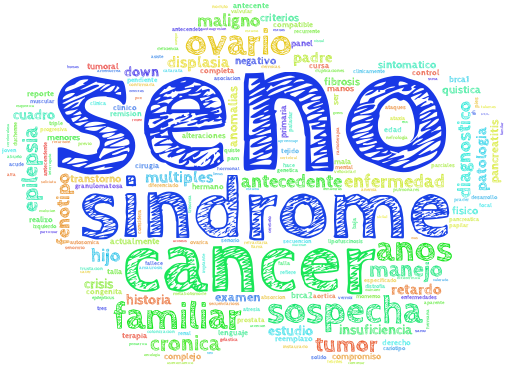
\includegraphics[width=70mm]{Kap4/cluster1}}
	\label{f:nube1}
	\subfigure[Distribucón demográfica de los pacientes]{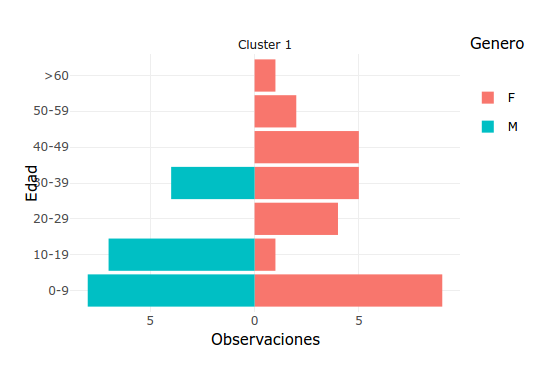
\includegraphics[width=70mm]{Kap4/edadc1}}
	\caption{Cluster 1} \label{fig:cluster1}
\end{figure} 

La figura \ref{fig:cluster1} representa el clúster 1 con la frecuencia de palabras que se agruparon para este clúster  la figura \ref{fig:cluster1}(a) se muestra la frecuencia de palabras, siendo seno,síndrome y cáncer son las palabras más frecuentes, junto con ovario,familiar sospecha y epilepsia. La figura \ref{fig:cluster1} representa la distribución de pacientes por edad y genero dentro del grupo por rango de edad en un intervalo de 10 años.\\

\begin{figure}[]
	\centering
	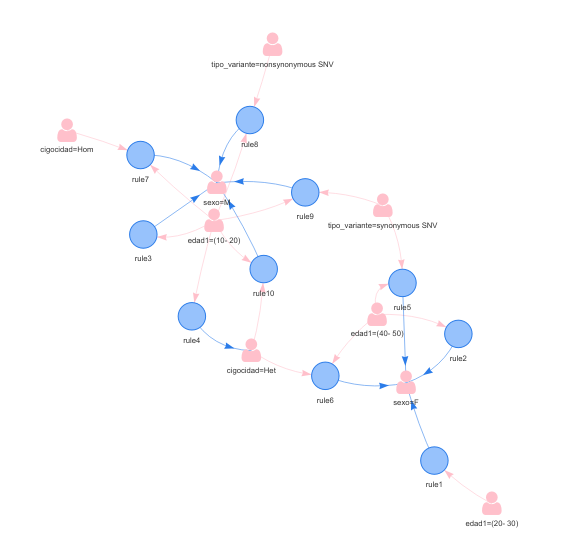
\includegraphics[width=0.5\textwidth]{Kap4/reglas1_1}
	\caption{Reglas de asociación del cluster 1 con variantes sinónimas} \label{fig:reglas1}
\end{figure}

Las primeras 10 reglas obtenidas se representan mediante la figura \ref{fig:reglas1} que muestra la asociación,sin remover las variantes sinónimas, el resultado obtenido muestra de dos tipos de variantes dentro del clúster 1. Para el genero masculino  se tiene que el tipo de variante es no sinónima, son pacientes de edad entre 10 y 20 años, el estado alélico de las variantes es homocigoto, para este grupo se observa una alta diferencia en las reglas ambos géneros.

\begin{figure}[H]
	\centering
	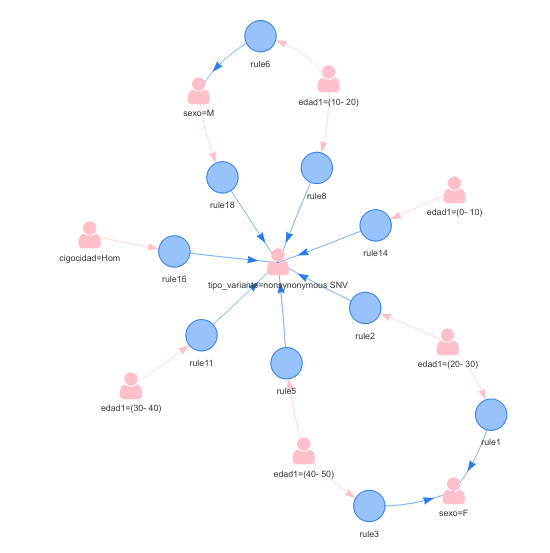
\includegraphics[width=0.5\textwidth]{Kap4/reglas1_2}
	\caption{Reglas de asociación del cluster 1 sin variantes sinónimas} \label{fig:reglas2}
\end{figure}


\subsubsection*{Cluster 2}

\begin{figure}[H]
	\centering
	\subfigure[Nube de palabras]{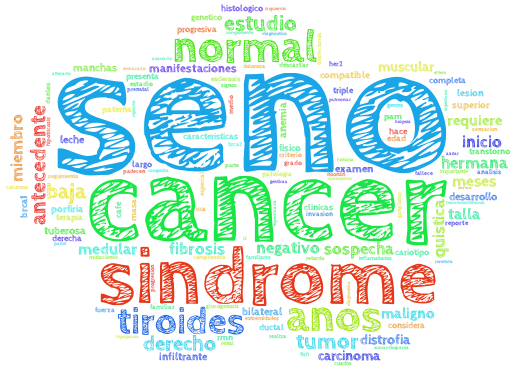
\includegraphics[width=60mm]{Kap4/cluster2}}
	\subfigure[Rango de edad en décadas.]{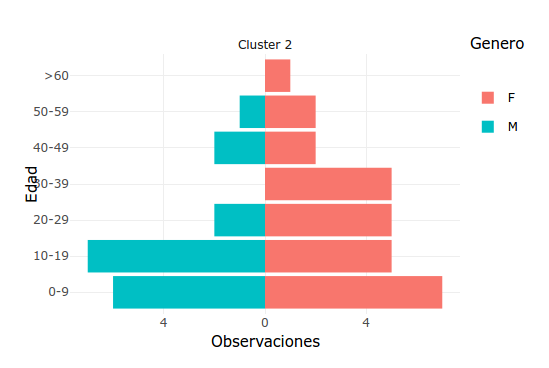
\includegraphics[width=60mm]{Kap4/edadc2}}
	\caption{Cluster 2} \label{fig:c2}
\end{figure}

\begin{figure}[H]
	\centering
	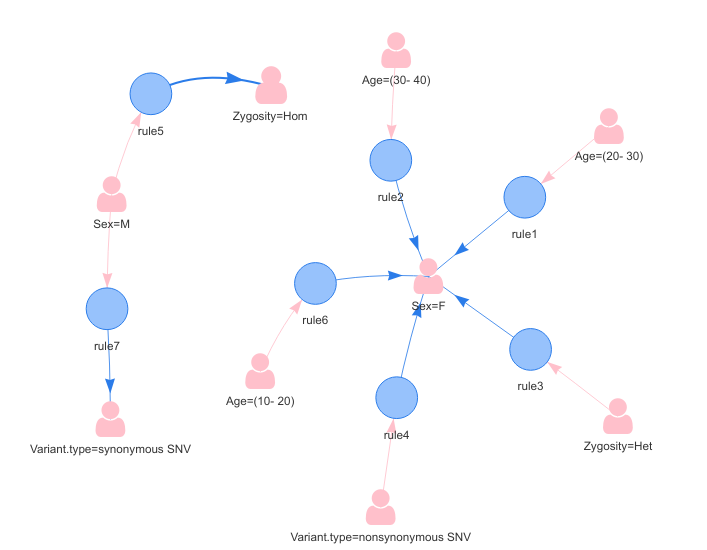
\includegraphics[width=0.5\textwidth]{Kap4/reglas2_1}
	\caption{Reglas de asociación del cluster 2 con variantes sinónimas} \label{fig:reglas2_1}
\end{figure}

\begin{figure}[H]
	\centering
	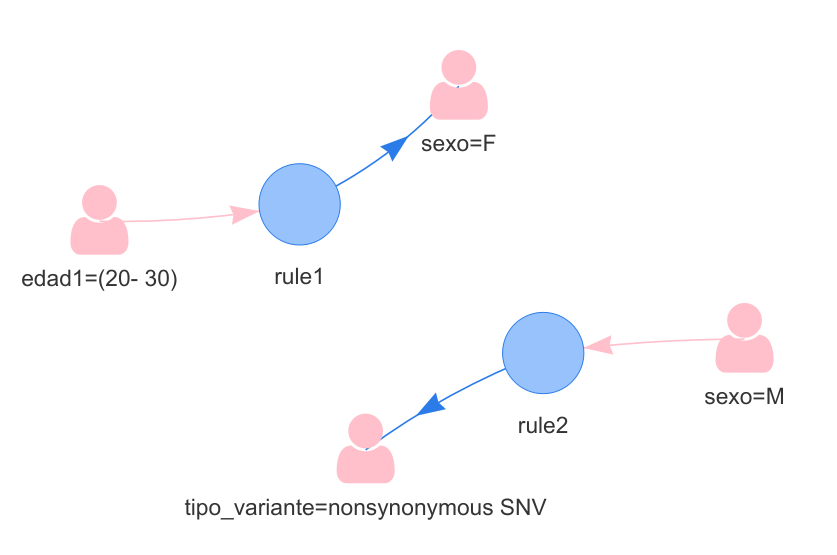
\includegraphics[width=0.5\textwidth]{Kap4/reglas2_2}
	\caption{Reglas de asociación del cluster 2 con variantes sinónimas} \label{fig:reglas2_2}
\end{figure}

\subsubsection*{Cluster 3}

\begin{figure}[H]
	\centering
	\subfigure[Nube de palabras]{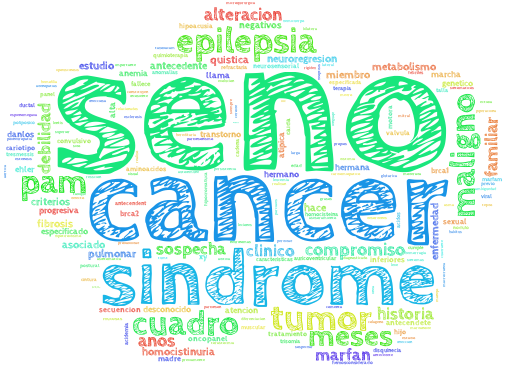
\includegraphics[width=60mm]{Kap4/cluster3}}
	\subfigure[Rango de edad en décadas.]{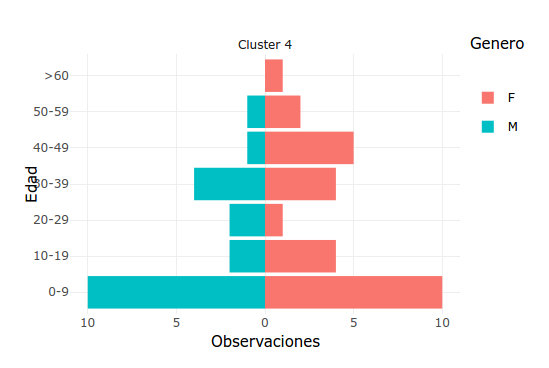
\includegraphics[width=60mm]{Kap4/edadc3}}
	\caption{Cluster 3} \label{fig:c3}
\end{figure}

\begin{figure}[H]
	\centering
	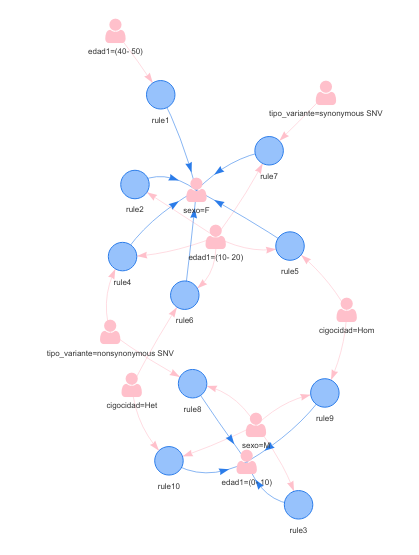
\includegraphics[width=0.5\textwidth]{Kap4/reglas3_1}
	\caption{Reglas de asociación del cluster 3 con variantes sinónimas} \label{fig:r3}
\end{figure}

\begin{figure}[H]
	\centering
	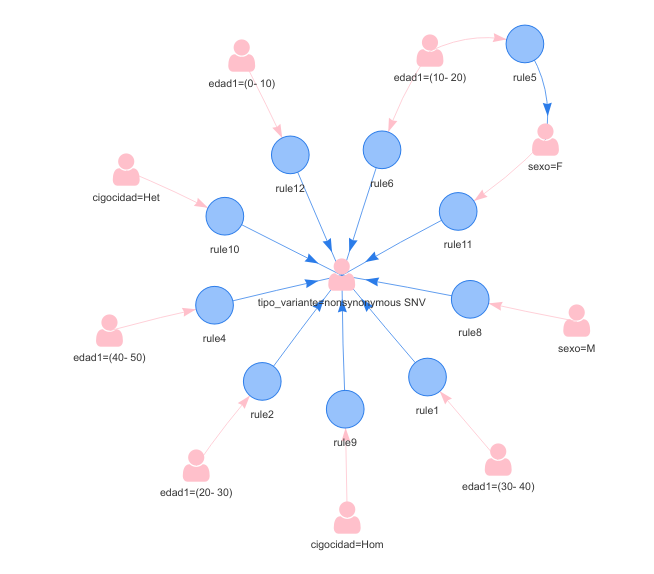
\includegraphics[width=0.5\textwidth]{Kap4/reglas3_2}
	\caption{Reglas de asociación del cluster 3 sin variantes sinónimas} \label{fig:r23}
\end{figure}

\subsubsection*{Cluster 4}
\begin{figure}[H]
	\centering
	\subfigure[Nube de palabras]{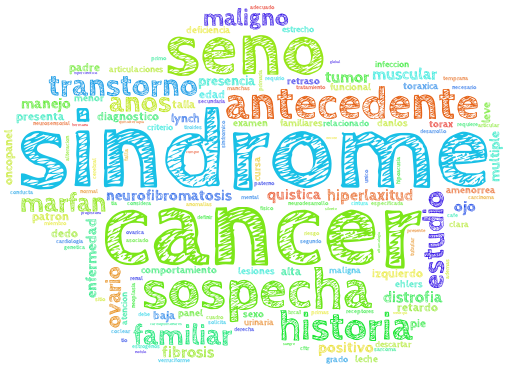
\includegraphics[width=60mm]{Kap4/cluster4}}
	\subfigure[Rango de edad en decadas]{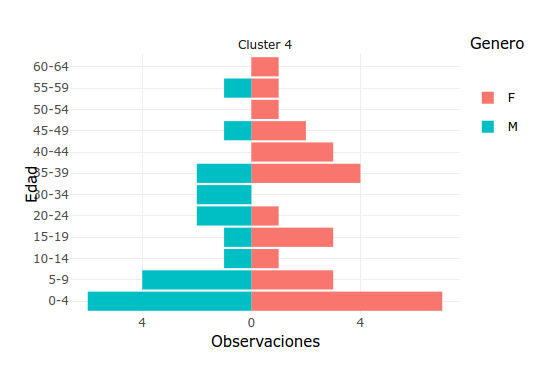
\includegraphics[width=60mm]{Kap4/edadc4}}
	\caption{Cluster 4} \label{fig:c4}
\end{figure}

\begin{figure}[H]
	\centering
	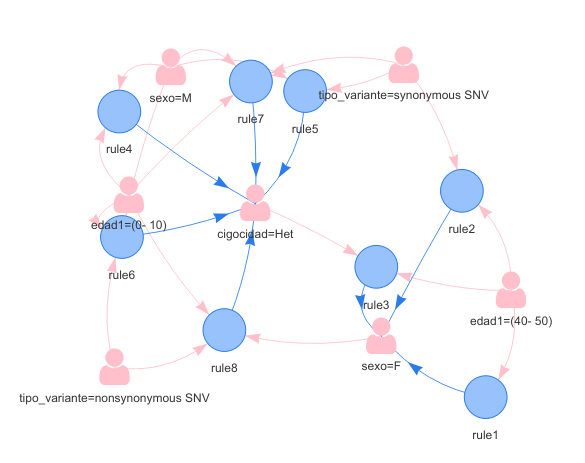
\includegraphics[width=0.5\textwidth]{Kap4/reglas4_1}
	\caption{Reglas de asociación del cluster 4 con variantes sinónimas} \label{fig:r4}
\end{figure}

\begin{figure}[H]
	\centering
	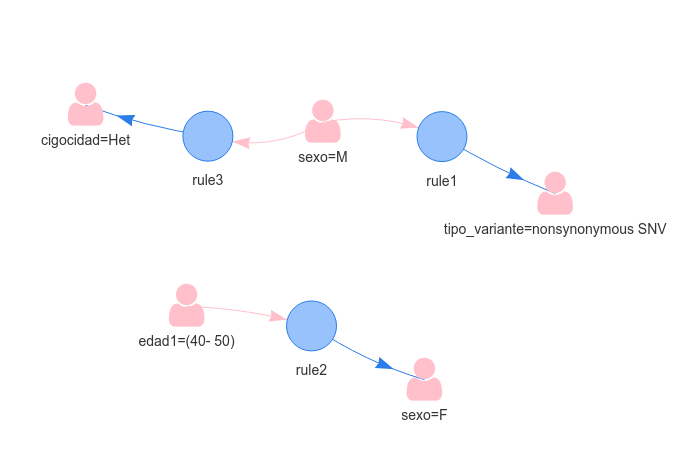
\includegraphics[width=0.5\textwidth]{Kap4/reglas4_2}
	\caption{Reglas de asociación del cluster 4 sin variantes sinónimas} \label{fig:re4}
\end{figure}

\subsubsection*{Cluster 5}

\begin{figure}[H]
	\centering
	\subfigure[Nube de palabras]{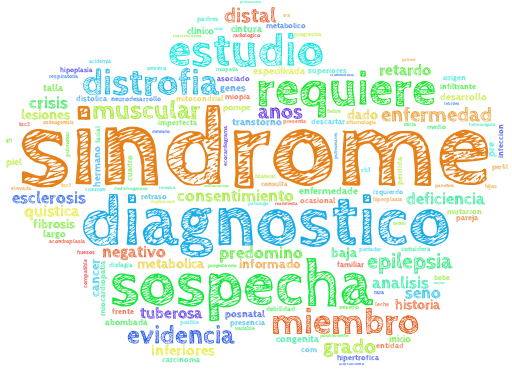
\includegraphics[width=60mm]{Kap4/cluster5}}
	\subfigure[Rango de edad en decadas]{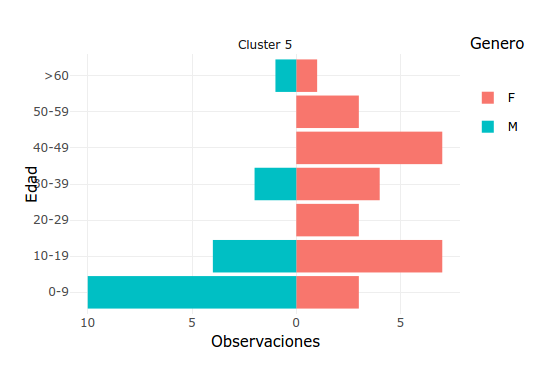
\includegraphics[width=60mm]{Kap4/edadc5}}
	\caption{Cluster 5} \label{fig:c5}
\end{figure}

\begin{figure}[H]
	\centering
	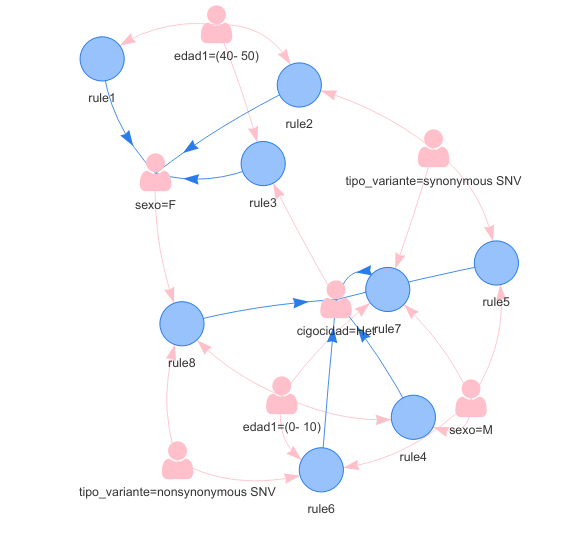
\includegraphics[width=0.5\textwidth]{Kap4/reglas5_1}
	\caption{Reglas de asociación del cluster 5 con variantes sinónimas} \label{fig:r5}
\end{figure}

\begin{figure}[H]
	\centering
	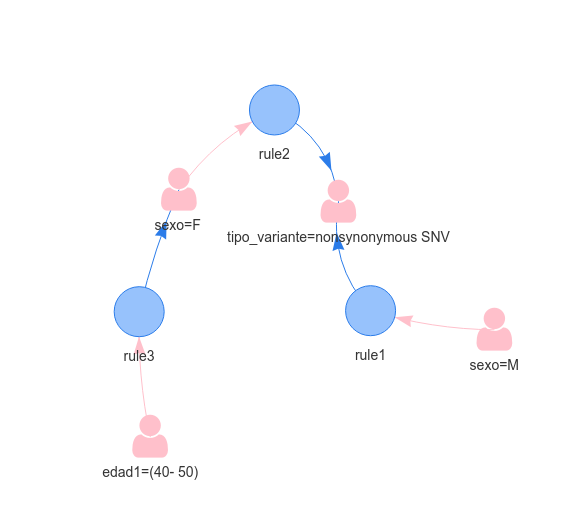
\includegraphics[width=0.5\textwidth]{Kap4/reglas5_2}
	\caption{Reglas de asociación del cluster 5 sin variantes sinónimas} \label{fig:re5}
\end{figure}

\subsubsection*{CFTR}

\begin{figure}[H]
	\centering
	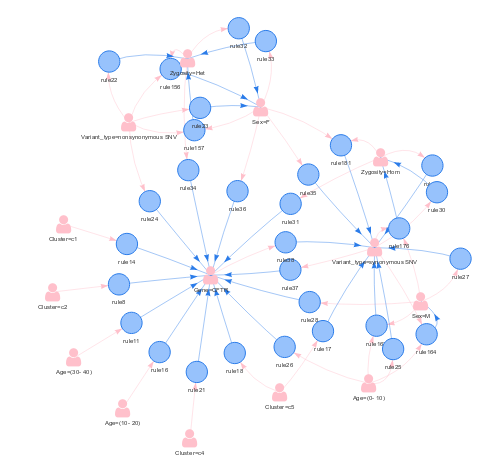
\includegraphics[width=0.5\textwidth]{Kap4/CFTR1}
	\caption{Reglas de asociación con variantes sinónimas} \label{fig:r6}
\end{figure}

\begin{figure}[H]
	\centering
	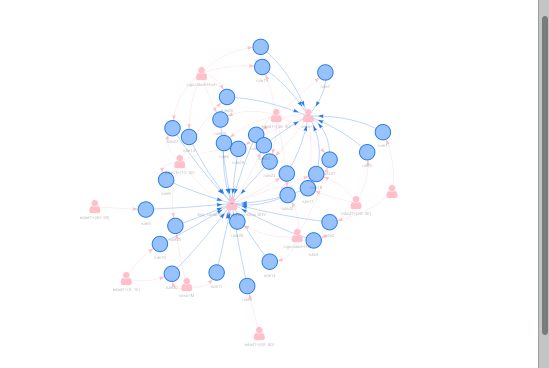
\includegraphics[width=0.5\textwidth]{Kap4/CFRT2}
	\caption{Reglas de asociación sin variantes sinónimas} \label{fig:r6}
\end{figure}